Les images à traiter sont bruitées, ne bénéficient pas de bonnes conditions d'éclairage et le support peut être de mauvaise qualité (pli de la feuille).\\
Avant de commencer la détection de nouveautés ou de formes, il est donc nécessaire de segmenter notre image afin de détecter les objets sur l'image.\\
Étant donné le type de support, un document avec des dessins noirs sur fond blanc, nous avons focalisé notre travail sur la binarisation ainsi que sur la détection de contours.

\paragraph{Binarisation par seuillage global\vspace{0.5cm}\\}

La binarisation à pour but de segmenter l'image en 2 classes, le fond et l'image.
Il existe différentes techniques pour binariser une image.

Nous avons choisi dans un premier temps un algorithme naïf de binarisation par seuillage global, on choisit la classe du pixel à partir d'un seuil.

\begin{equation}
	\forall i,j \in \mathbf{M*N} \quad I(i,j)=
	\left\lbrace
	\begin{array}{ccc}
		1 &\mbox{si}& f(i,j) > S,\\
		0 &\mbox{sinon}&
	\end{array}\right.
\end{equation}
Avec : \\
$\mathbf{M*N}$ nombre de colonnes et de lignes de l’image ;\\
$I$ image binarisée ;\\
$S$ seuil de binarisation.\\
$f$ valeur fonction de l’image d’origine ;\\


Le problème est que l'on utilise des documents dégradés (mauvaise illumination et papier marqué) donc bien souvent il n'existe pas de seuil global.

\begin{center}
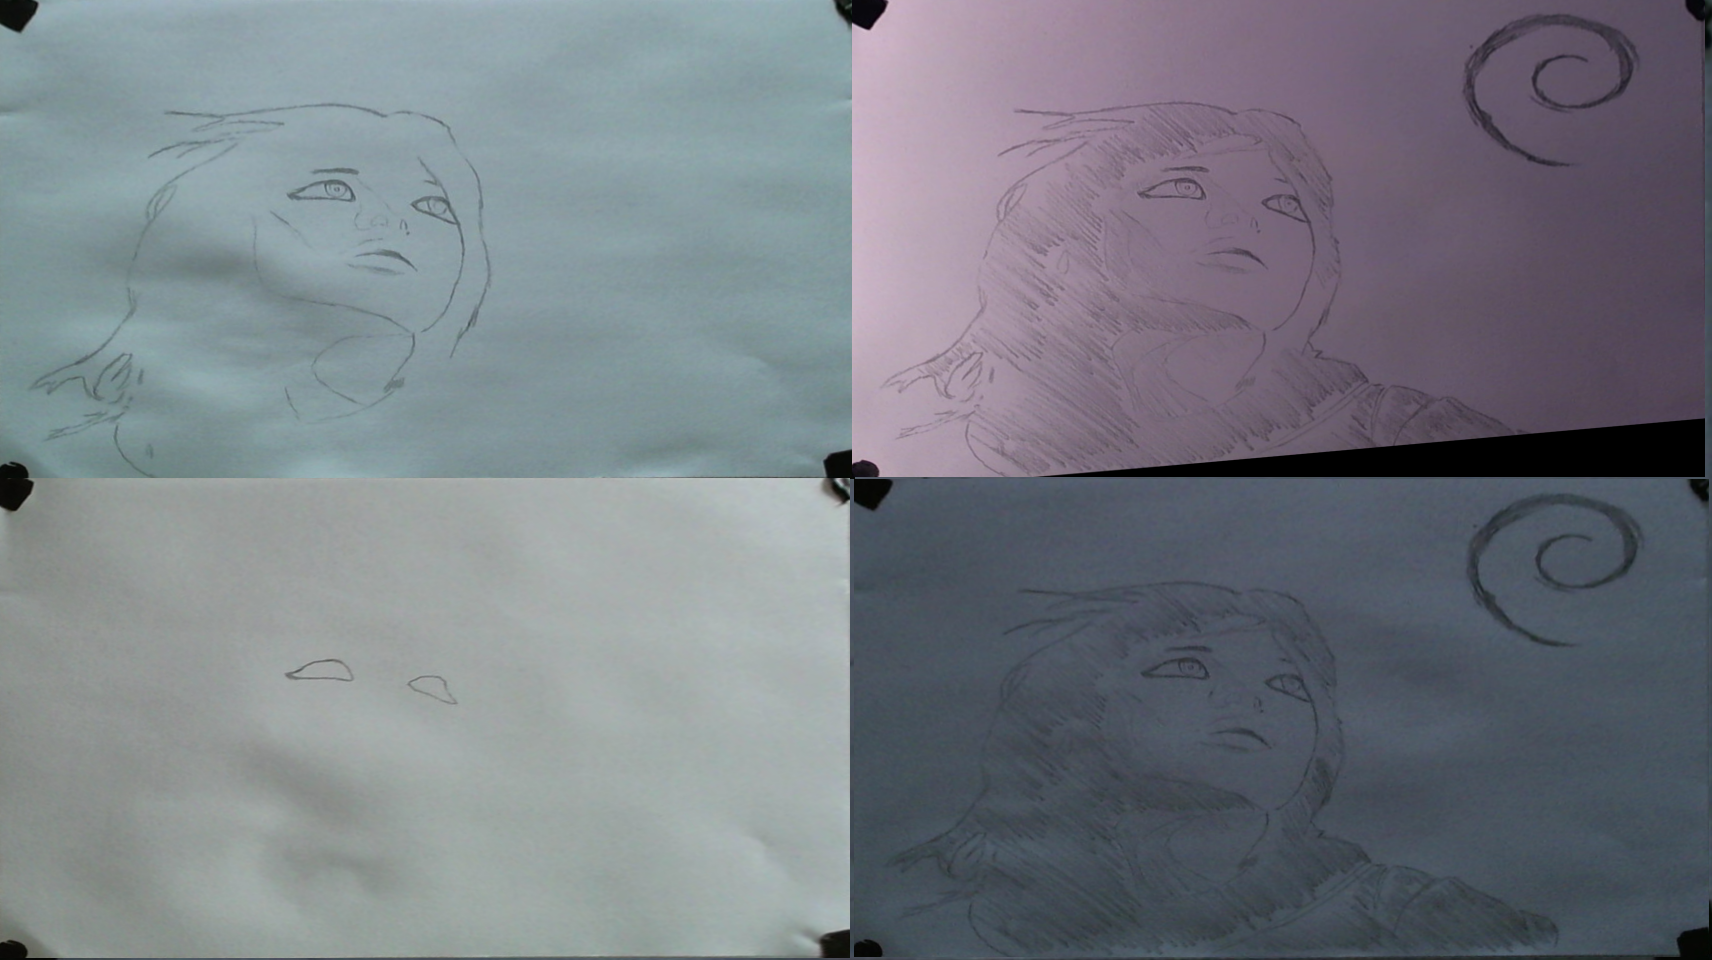
\includegraphics[width=\textwidth]{images/diffEclairage.png}
\captionof{figure}{Différence d'eclairage}
\end{center}

Pour corriger l'illumination, nous avons appliqué une balance des blancs basée sur l'étirement de l'histogramme de chaque canal de l'image.

\begin{center}
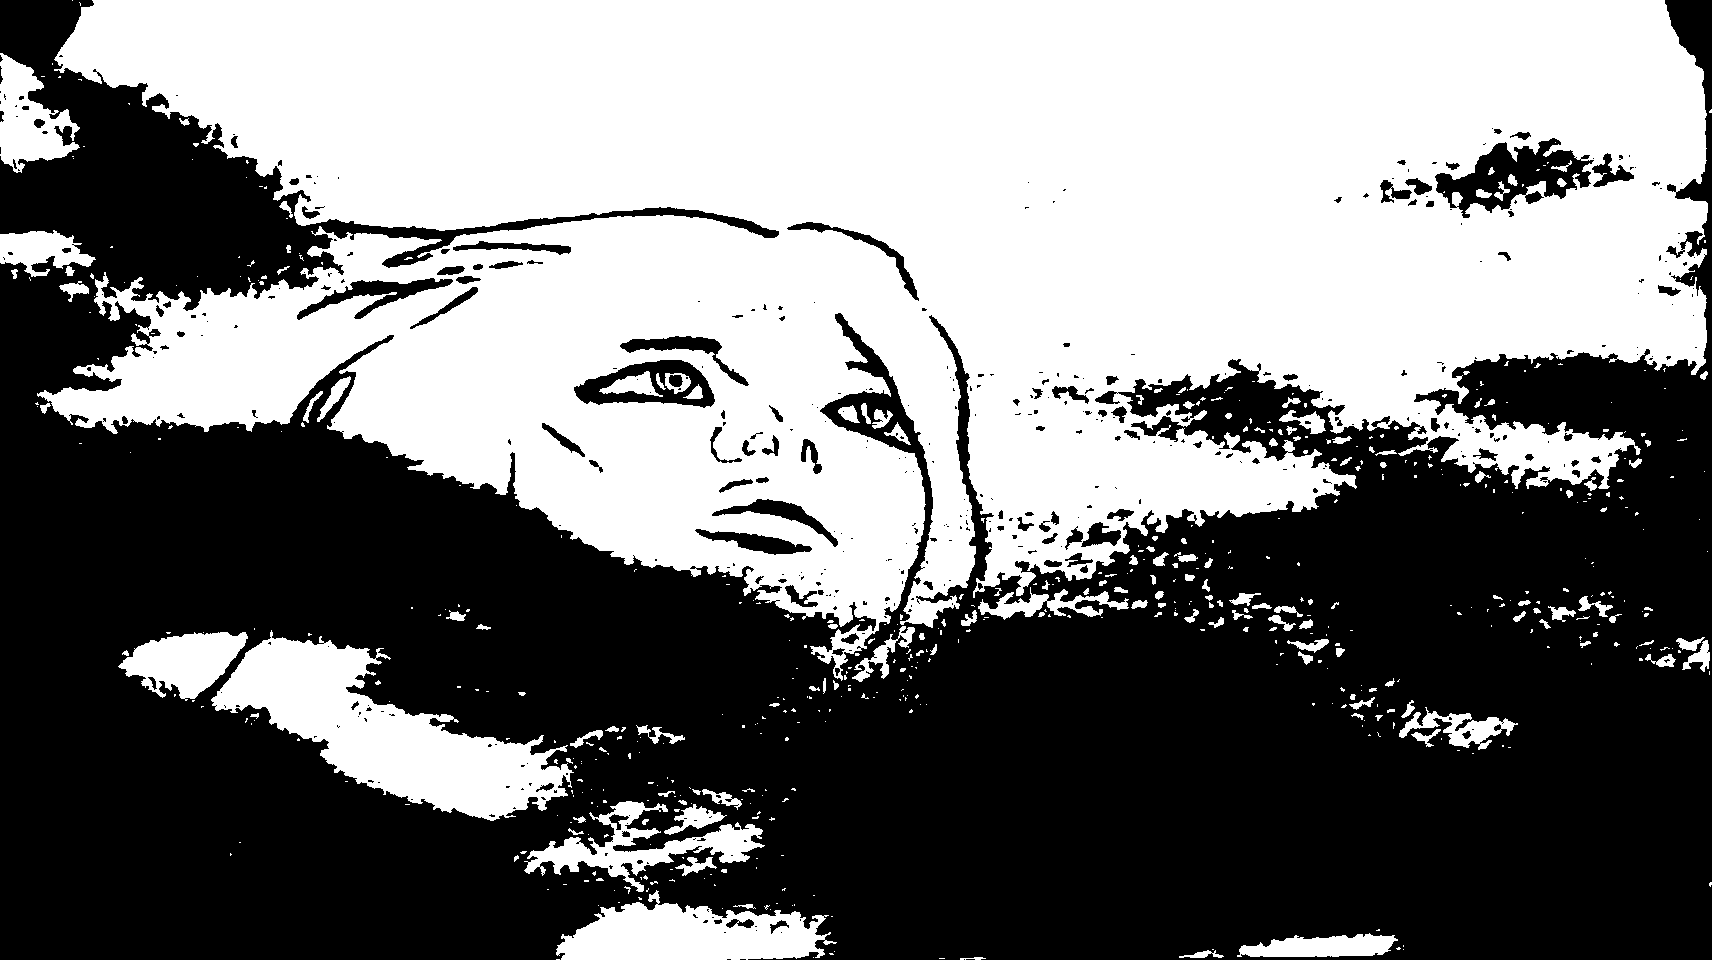
\includegraphics[width=\textwidth]{images/Threshold.png}
\captionof{figure}{Résultat seuillage global}
\end{center}

\paragraph{Binarisation par détection de contour\vspace{0.5cm}\\}

Il existe de nombreuses méthodes de détection de contour, nous avons appliqué le filtre de sobel.
Il s'agit d'appliquer deux matrices de convolution $G_x$ $G_y$ à l'image qui calculent la dérivée verticale et horizontale. 
\[ G_x = \left| \begin{array}{ccc}
+1 & 0 & -1 \\
+2 & 0 & -2 \\
+1 & 0 & -1 \end{array} \right|.\] 

\[ G_y = \left| \begin{array}{ccc}
+1 & +2 & +1 \\
0 & 0 & 0 \\
-1 & -2 & -1 \end{array} \right|.\] 

Puis, il faut calculer en chaque point une approximation de la norme du gradient. 
\[ G = \sqrt{G_x^2 - G_y^2} \]


Les résultats étaient bien sur efficaces sur les traits fins mais moins bons dans les zones homogènes (coloriées)
Toutefois il est possible d'obtenir un masque des zones contenant un objet, en y combinant des filtres morphologiques et un seuillage global.
Voici les étapes de notre binarisation :

\begin{itemize}
   \item Flou Gaussien. (lissage pour atténuer le bruit) 
   \item Sobel
   \item Fermeture morphologique (pour éliminer le bruit produit par sobel)
   \item Ouverture pour combler les trous de l'objet 
   \item Binarisation seuillage global
\end{itemize} 

\begin{center}
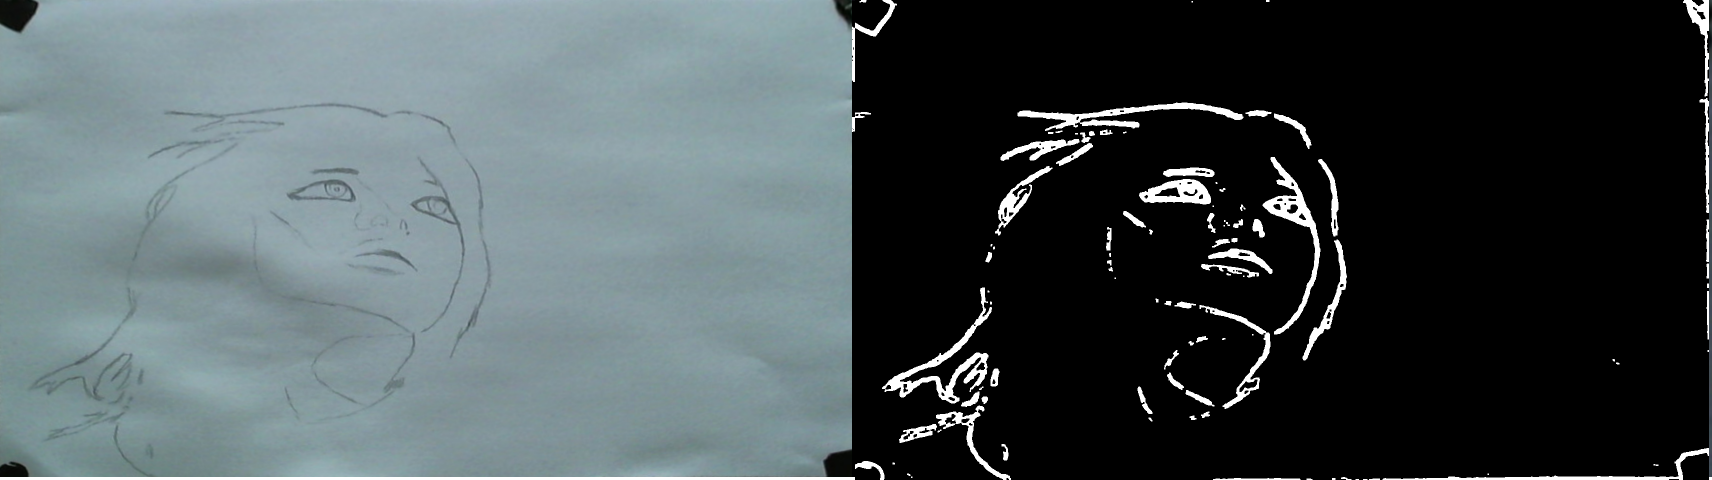
\includegraphics[width=\textwidth]{images/sobelComp.png}
\captionof{figure}{Résultat masque par binarisation par détection de contour}
\end{center}


\paragraph{Autres méthodes de Binarisation\vspace{0.5cm}\\}


L'étude \cite{Mehmet04}, compare et classe les différents algorithmes de binarisation pour les images dégradées.

La méthode de Kittler \cite{Kittler86} se basant sur le clustering, nous avons abandonné cette méthode car les résultats obtenus étaient insuffisants.

Un autre type de méthode de binarisation contient les méthodes par seuillage local, leur principe est d’utiliser une étude localisée autour du pixel pour déterminer quel seuil utiliser. Pour réaliser cette étude locale, les techniques utilisent une fenêtre d’étude centrée sur le pixel à étudier. Cette fenêtre peut avoir différentes tailles, de nombreuses méthodes ont été proposées : Bernsen \cite{JB86}, Niblack \cite{Nib86}, Sauvola\cite{Sauvola00}.

Sauvola est indiqué comme obtenant les meilleurs résultats.

\begin{equation}
	S(i,j) = \mu(i,j) + \kappa.((\sigma(i,j)/R)-1))
\end{equation}

Avec :
- S(i, j) : seuil à appliquer pour le point i, j ;\\
- $\sigma(i, j)$ : valeur de l’écart-type dans une fenêtre centré en i, j de taille $N * M$ ;\\
- $\mu(i, j)$ : valeur moyenne des niveaux de gris dans la même fenêtre ;\\
- $\kappa$ : constante fixée le plus généralement à 0, 2 ;\\
- $R$ : constante permettant d'ajuster la dynamique de l’écart-type, généralement 128.
- $N$ et $M$ appartenant à $\mathbb{N}$.\\

La méthode de Sauvola calcule le seuil de binarisation en fonction de la moyenne et de l’écart-type des pixels ajusté par la constante $R$, le rapport entre les deux est défini par la constante $\kappa$.
Sauvola conseille un $\kappa \in \left[ 0.2 ;0.5 \right]$, mais ce type de paramètre est fixé pour binariser des textes, or nos documents sont des dessins effectués au crayon à papier et peuvent avoir des traits très fins.

Nous fixons $\kappa$ à 0.05, ce qui augmente l'influence de l’écart-type et permet d'obtenir de meilleurs résultats, notamment lorsqu'il y a un faible contraste comme dans notre cas.   

Une optimisation possible de la méthode de binarisation Sauvola passe par l'utilisation des images intégrales présentées dans \cite{Viola04}

Les images intégrales sont une représentation sous la forme d'une image, de même taille que l'image d'origine, qui en chacun de ses points contient la somme des pixels situés au dessus et à gauche de ce point. Plus formellement, l'image intégrale $ii$ est définie à partir de l'image $i$ par : 

\begin{equation}
	ii(x,y) = \sum_{x' \leq x  \atop y' \leq y } i(x',y')
\end{equation}

\begin{center}
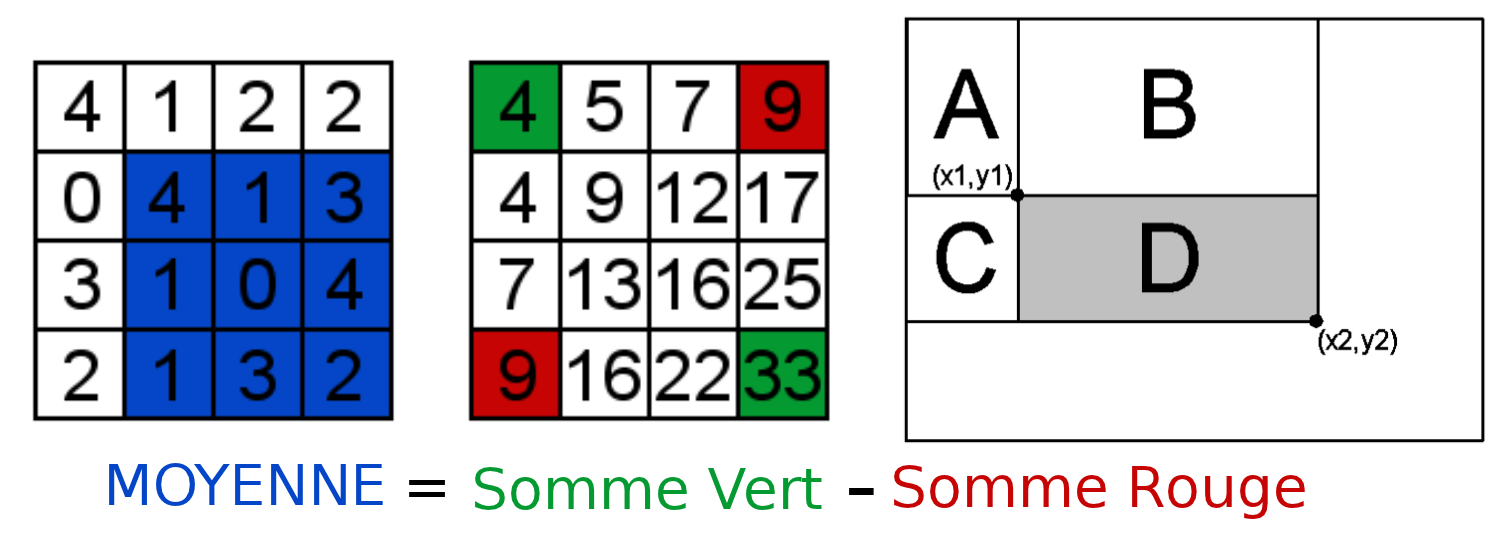
\includegraphics[width=\textwidth]{images/imageIntegrale.png}
\captionof{figure}{A gauche une image simple, au centre l'image intégrale, et à droite le calcul de la zone D avec l'image intégrale \cite{BradleyRoth07}}
\end{center}

Ainsi on peut calculer la moyenne d'un rectangle en deux additions et deux soustractions par :

\begin{equation}
	I(x, y) = f (x, y) + I(x - 1, y) + I(x - 1) - I(x - 1, y - 1)
\end{equation}

\begin{center}
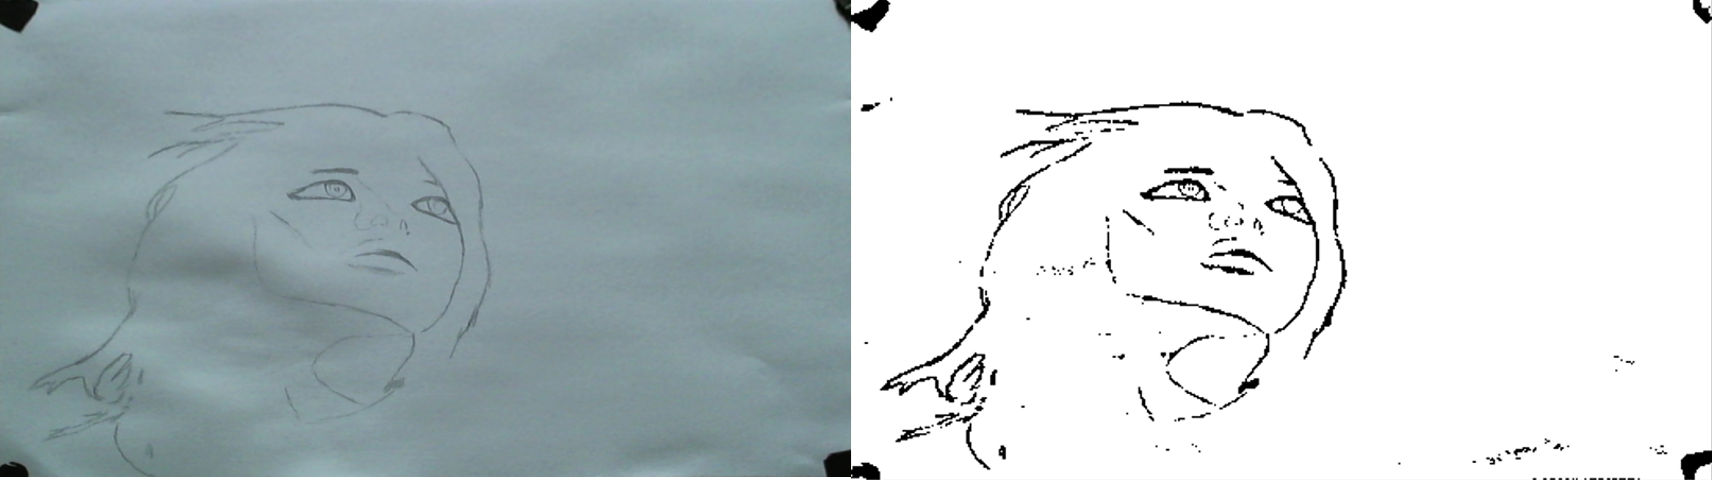
\includegraphics[width=\textwidth]{images/sauvola.png}
\captionof{figure}{Méthode de Sauvola}
\end{center}

\paragraph{Bilan comparatif des méthodes\vspace{0.5cm}\\}

\begin{center}
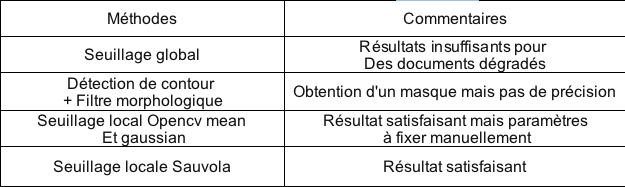
\includegraphics[width=\textwidth]{images/methodescommentaire.png}
\captionof{figure}{Tableau de bilan}
\end{center}

La méthode de seuillage local de Sauvola\cite{Sauvola00} se trouve être la solution la plus appropriée à nos besoins.
C'est la méthode que nous utilisons en pré-traitement pour la reconnaissance de formes et de nouveautés.   